\chapter{Physical Problem}
\label{PhysicalProblemChapter}
\lhead{Chapter 2. \emph{Physical Problem}} In this chapter, Maxwell's equations
of classical electrodynamics are introduced, both in integral and in differential
forms. The wavelengths considered are assumed to be sufficiently large, with respect to
atomic scale variations in the medium, that a macroscopic approach is justified
and quantum mechanical effects are neglected. Constitutive equations will be
introduced for linear, isotropic material both with and without dispersive
effects. Following this, the Drude model is introduced and used to incorporate
frequency-dependent interactions into Maxwell's equations in a formulation
suitable for efficient numerical calculation. The conditions which must be
satisfied at material interfaces will be derived and alternative forms of
Maxwell's equations discussed.

\section{Maxwell's equations}
The classical theory of electrodynamics decribes the behaviour of
electromagnetic radiation using Maxwell's unification of the equations of
electrodynamics~\cite{Balanis:ui,Jackson:490457}. The resulting coupled
equations, which govern the time evolution of electromagnetic waves, are known
collectively as Maxwell's equations, and written in standard units as
\begin{subequations}
  \begin{align}
    \int_{\partial S} \Etilde(\xbftilde,\ttilde) \cdot \vectdl  &= - \dodettilde{} \int_{S} \Btilde(\xbftilde,\ttilde) \cdot \vectdS, \label{eq:maxwell-faraday-integral} \\
    \int_{\partial S} \Btilde(\xbftilde,\ttilde) \cdot \vectdl &= \mu_0 \eps_0 \dodettilde{} \int_{S} \Etilde(\xbftilde,\ttilde) \cdot \vectdS +  \mu_0 \int_{S} \Jtilde(\xbftilde,\ttilde) \cdot \vectdS, \label{eq:maxwell-ampere-integral} \\
    \int_{\partial \Vol} \Dtilde(\xbftilde,\ttilde)\cdot\vectdS &= \int_\Vol \rho \,\dV, \label{eq:maxwell-gauss-integral} \\
    \int_{\partial \Vol} \Btilde(\xbftilde,\ttilde)\cdot\vectdS &= 0, \label{eq:maxwell-gauss-magnetism-integral}
  \end{align}
\end{subequations}
where $\xbftilde$ is the position vector, $\ttilde$ is time in seconds, $\eps_0$
is the permittivity of free space in farads per meter, $\mu_0$ is the
permeability of free space in henries per meter and the vectors $\Etilde$,
$\Htilde$, $\Dtilde$ and $\Btilde$ are used to denote respectively the electric
field intensity in volts per meter, magnetic field intensity in amps per meter,
electric displacement in coulombs per meter squared, and magnetic induction in
weber per meter squared. $\rho$ denotes volume charge density in coloumbs per
meter cubed and $\Jtilde$ denotes electric current density in ampere per meter
squared.
% VIVA: these are BOTH due to EXTERNAL charge only, this means not due to induced effects (e.g polarisation) QUOTE: both denote sources due to free charges in the system
% TODO: maybe I should mention these are free charges? is that the correct terminology
$\Vol$ denotes any closed volume while the infinitesimal integration elements
$\vectdl$, $\vectdS$ and $\dV$ are respectively a line element, vector surface
element and volume element.
% "In regions where the material parameters are differentiable"... -> but hang on! The material parameters are not involved here. What restrictions are the for using Stokes' Theorem?
By applying Stokes' Theorem to~\eqref{eq:maxwell-faraday-integral}
and~\eqref{eq:maxwell-ampere-integral} and Gauss' law
to~\eqref{eq:maxwell-gauss-integral}
and~\eqref{eq:maxwell-gauss-magnetism-integral}, the equations in differential
form are obtained as
\begin{subequations}
  \label{eq:maxwells-equations-diff}
  \begin{align}
    \nablatilde \times \Etilde(\xbftilde,\ttilde) + \dpartttilde{\Btilde(\xbftilde, \ttilde)}&= \mathbf{0}, \label{eq:maxwell-faraday} \\
    \nablatilde \times \Htilde(\xbftilde,\ttilde) - \dpartttilde{\Dtilde(\xbftilde, \ttilde)}&= \Jtilde(\xbftilde,\ttilde), \label{eq:maxwell-ampere} \\
    \nablatilde \cdot \Dtilde (\xbftilde,\ttilde) &= \rho(\xbftilde,\ttilde), \label{eq:maxwell-gauss-1} \\
    \nablatilde \cdot \Btilde (\xbftilde,\ttilde) &= 0, \label{eq:maxwell-gauss-2} 
  \end{align}
\end{subequations}
where $\nablatilde = \left( \dpart{}{\xtilde_1}, \dpart{}{\xtilde_2}, \dpart{}{\xtilde_3} \right)$ denotes the nabla operator. The four equations in~\eqref{eq:maxwells-equations-diff} are known respectively as Ampere's law with Maxwell's correction, Faraday's law, Gauss' law and Gauss' law for magnetism. Equations~\eqref{eq:maxwell-ampere} and~\eqref{eq:maxwell-faraday} determine the evolution of the vector fields in time, and are referred to as Maxwell's curl equations. Equations~\eqref{eq:maxwell-gauss-1} and~\eqref{eq:maxwell-gauss-2} are constraints referred to as Maxwell's divergence conditions.

\subsection{Conservation of charge}
Conservation of charge can be derived directly from Maxwell's equations. Taking the divergence of both sides of Ampere's law,~\eqref{eq:maxwell-ampere}, and using the vector identity
\begin{equation}
  \label{eq:vector-identity-1}
  \nablatilde \cdot ( \nablatilde \times \mathbf{A} (\xbftilde) ) = 0,
\end{equation}
which holds for any vector field $\mathbf{A}$, gives
\begin{equation}
- \dpartttilde{( \nablatilde \cdot \Dtilde(\xbftilde,\ttilde) ) } = \nablatilde \cdot \Jtilde(\xbftilde,\ttilde) . \label{eq:maxwell-conservation-charge-eq1}
\end{equation}
By substituting Gauss' law,~\eqref{eq:maxwell-gauss-1}, into~\eqref{eq:maxwell-conservation-charge-eq1} the following conservation equation for charge is obtained
\begin{equation}
  \nablatilde \cdot \Jtilde(\xbftilde,\ttilde) + \dpartttilde{\rho (\xbftilde,\ttilde) } = 0 .
  \label{eq:maxwell-charge-conservation-2}
\end{equation}
Taking the divergence of Amperes law,~\eqref{eq:maxwell-ampere}, and removing
the curl term by recalling the identity~\eqref{eq:vector-identity-1}, results in
$$
\nablatilde \cdot \dpartttilde{ \Dtilde(\xbftilde, \ttilde)} = - \nablatilde
\cdot \Jtilde(\xbftilde,\ttilde),
$$
which can be rewritten using the conservation of charge
equation,~\eqref{eq:maxwell-charge-conservation-2}, as
$$
\dpartttilde{} \left(  \nablatilde \cdot \Dtilde(\xbftilde, \ttilde) +  \rho (\xbftilde,\ttilde) \right)  = 0.
$$
Following a similar procedure using~\eqref{eq:maxwell-faraday} results in
$$
\dpartttilde{} \left(\nablatilde \cdot  \Btilde(\xbftilde, \ttilde)\right) = 0 
$$

Thus given initial conditions which satisfy both Maxwell's divergence
conditions,~\eqref{eq:maxwell-gauss-1} and~\eqref{eq:maxwell-gauss-2}, and given
that conservation of charge,~\eqref{eq:maxwell-charge-conservation-2}, is
satisfied at all times, then solutions to Maxwell's curl equations 
implicitly satisfy the divergence conditions at all times.

\section{Constitutive equations}
\label{Ch:PhysicalProblem:ConstitutiveEquations}
Maxwell's equations in differential form,~\eqref{eq:maxwells-equations-diff},
are an underdetermined system of equations, in which 4 equations involve 6 unknowns. The
system of equations is closed by a set of macroscopic constitutive laws, which
account for the behaviour of the medium, and are written as
% VIVA: this is not true for materials which exhibit ferromagnetic or
% ferroelectric behaviour - but this is a quantum effect, so outside of our
% classical scope. what are the constitutive laws in this case?
\begin{subequations}
  \begin{align}
    \Dtilde(\xbftilde,\ttilde) &= \eps_0 \Etilde(\xbftilde,\ttilde) + \Ptilde  \label{eq:constitutive-general-E}\\
    \Btilde(\xbftilde,\ttilde) &= \mu_0 \Htilde(\xbftilde,\ttilde) + \Mtilde \label{eq:constitutive-general-H}
  \end{align}
\end{subequations}
where $\Ptilde$, the polarisation density, and $\Mtilde$, the magnetisation density, are vectors describing the induced fields in the medium.
% However, for a given material the dependence may be non-local in space,
% non-local in time, non-linear, and/or anisotropic.
The polarisation and magnetisation densities of linear, isotropic media and time-invariant media are described by
\begin{subequations}
  \begin{align}
    \Ptilde &= \eps_0 \ElecSuccept(\xbftilde) \Etilde(\xbftilde,\ttilde), \label{eq:elec-susceptibilities-definition-E} \\
    \Mtilde &= \eps_0 \MagSuccept(\xbftilde) \Htilde(\xbftilde,\ttilde) . \label{eq:elec-susceptibilities-definition-H} 
  \end{align}
\end{subequations}
where $\ElecSuccept$, the electric suceptibility, and $\MagSuccept$, the magnetic susceptibility, are proportionality constants between the applied and induced fields. Substitution of~\eqref{eq:elec-susceptibilities-definition-E} and~\eqref{eq:elec-susceptibilities-definition-H} into~\eqref{eq:constitutive-general-E} and~\eqref{eq:constitutive-general-H} results in
\begin{subequations}
  \begin{align}
    \Dtilde(\xbftilde,\ttilde) = \eps_0 \left( 1 + \ElecSuccept(\xbftilde)  \right) \Etilde(\xbftilde,\ttilde), \\
    \Btilde(\xbftilde,\ttilde) = \mu_0  \left( 1 + \MagSuccept(\xbftilde) \right)  \Htilde(\xbftilde,\ttilde).
  \end{align}
\end{subequations}

By introducing two dimensionless scalars which characterise the material response, $\eps_r \equiv 1 + \ElecSuccept $ and $\mu_r \equiv 1 + \MagSuccept $, respectively the relative permittivity and permeability, the constitutive equations are given by
\begin{subequations}
  \label{eq:constitutive-linear}
  \begin{align}
    \Dtilde(\xbftilde,\ttilde) = \eps_0 \eps_r(\xbftilde) \Etilde(\xbftilde,\ttilde), \label{eq:constitutive-linear-D} \\
    \Btilde(\xbftilde,\ttilde) = \mu_0 \mu_r(\xbftilde) \Htilde(\xbftilde,\ttilde),\label{eq:constitutive-linear-B}
  \end{align}
\end{subequations}
% TODO - cite{Maier:5SXqSjV8} -> copied

\subsection{Dispersive Drude Media}
Most media exhibit some variation of both $\eps_r$ and $\mu_r$ with frequency. This
phenomena, known as dispersion, arises due to the finite time charged particles
need to reach equilibrium states in the presence of a time-varying electromagnetic field.
Whilst dispersive effects are generally neglected in simulations of dielectrics, many metals of
interest in photonics, such as gold, silver and aluminum, have strongly
frequency dependent relative permittivities in the visible and infra-red regions
of the electromagnetic spectrum~\cite{Ordal:1983bg}. In such cases, the electric susceptibility can no longer be written as a function of
$\xbftilde$ only, but is expressed as a convolution integral in time~\cite{Jackson:490457}.
% VIVA: article - A comparison of numerical techniques for modeling well
For metals where the effects of interband electron transitions are negligible, a
mechanical model based on the Drude model of solids is
sufficient~\cite{taflove2013advances}. For more complex material interactions
however, a more sophisticated model such as the Drude-Lorentz
model~\cite{Fox:2001wm,Taflove:1989ds} or approaches based on the
$Z$-transform~\cite{sullivan1996z} may be used. In this work, all media have frequency-independent magnetisation, thus~\eqref{eq:constitutive-linear-B} remains valid,
and have a polarisation which is well approximated by a single-pole Drude model.

%% *** ## "Polarisation density also describes how a material responds to an
%% applied electric field as well as the way the material changes the electric
%% field, and can be used to calculate the forces that result from those
%% interactions."
% ...based on the kinetic theory of gases,
%
% *** "The induced polarisation due to frequency-dependent electron movement
% leads to a frequency-dependent polarisation (dispersion)" - ref Maier
%
% Electron-ion collisions are random events, with a probability $dt / \tau$ (tau
% is the inv of gamma) - following which the electron velocities are independent
% of velocities prior to collision.
A Drude medium is composed of a lattice of fixed-position, positively charged
ions bound by a delocalised sea of valence band free
electrons~\cite{Ashcroft:2005wp,Bandyopadhyay:1503732}. The free electrons,
following the kinetic theory of ideal gases, are non-interacting, independent
particles, described by Newtonian mechanics. In the presence of the electric
field, $\Etilde$, the ions remain fixed and only the free electrons are
displaced from their zero-field equilibrium positions. In the Drude model
polarisation arises from two independent sources: a frequency-independent
background polarisation, $\PtildeInf$, due to the fixed-position charged ions,
and a frequency dependent free electron polarisation, $\PtildeElec$, due to the
delocalisation of free electrons in the presence of an electric field. Thus~\eqref{eq:constitutive-general-E} is rewritten in the frequency domain as
\begin{align}
  \hat{\Dtilde}(\xbftilde,\omega) &= \eps_0 \hat{\Etilde}(\xbftilde, \omega) + \PtildeInfFreq + \PtildeElecFreq(\xbftilde,\omega) ,
                                    \label{eq:constitutive_equations_drude_model}
\end{align}
where $\omega$ is the frequency variable and a circumflex denotes the frequency
domain representation of a time domain quantity, such that
$$
\hat{\Box}(\xbftilde,\omega) = \int_{-\infty}^{+\infty} \Box(\xbftilde,\ttilde)
e^{-i \omega t} dt
$$
where the real-valued function $\Box$ of the temporal variable, $\ttilde \in
\Real$, is written as the complex valued function $\hat{\Box}$ of angular
frequency, $\omega \in \Real$.
%, which is related to frequency, $f$, by $\omega = 2 \pi f$.
Note in particular that $- i \omega \hat{\Box}(\xbftilde,\omega) =
\dpartt{ \Box(\xbftilde,\ttilde) }$.

Since $\PtildeInfFreq$ is frequency-independent, following the procedure
from~\autoref{Ch:PhysicalProblem:ConstitutiveEquations}, equation~\eqref{eq:constitutive_equations_drude_model} is rewritten as
\begin{equation}
  \hat{\Dtilde}(\xbftilde,\omega) = \eps_0 \eps_{\infty} \hat{\Etilde}(\xbftilde, \omega) + \hat{\Ptilde}_e(\xbftilde,\omega) ,
\end{equation}
where $\eps_{\infty} \equiv 1 + \ElecSucceptInf $ is the permittivity in the
infinite frequency limit, and $\ElecSucceptInf$ is defined by $\PtildeInfFreq = \eps_0 \ElecSucceptInf \hat{\Etilde} $.
% TODO F - eleborate on this paragraph - are there other options
Transforming~\eqref{eq:constitutive_equations_drude_model} directly to the time domain would lead to a convolution integral, which presents challenges for numerical simulation~\cite{kelley1996piecewise}. Instead, the so called auxiliary differential equation (ADE) approach~\cite{Taflove:1989ds,Stannigel:09, Ji:2007dl,okoniewski1997simple,kashiwa1990treatment}, is followed.
% end elaboration
First the current due to free electron polarisation is defined as,
\begin{align}
  \Jtildep(\xbftilde,\ttilde) =  \dpartttilde{\Ptilde_e(\xbftilde,\ttilde)}. \label{eq:polarisation-current-definition}
\end{align}
By multiplying~\eqref{eq:constitutive_equations_drude_model} by $ -i \omega$ and
then transforming it to the time domain, a constitutive relation in
the form of an ordinary differential equation is obtained,
\begin{equation}
  \label{eq:constitutive_equations_drude_model_derivative_TD}
  \dodettilde{ \Dtilde (\xbftilde,\ttilde) }= \eps_0 \eps_{\infty} \dodettilde{ \Etilde (\xbftilde, \ttilde) } + \Jtildep(\xbftilde,\ttilde) .
\end{equation}
Substitution into Ampere's law,~\eqref{eq:maxwell-ampere}, results in
\begin{align}
  \nablatilde \times \Htilde(\xbftilde,\ttilde) - \dpartttilde{\Dtilde_{\infty}(\xbftilde, \ttilde)} &= \Jtilde(\xbftilde,\ttilde) + \Jtildep(\xbftilde,\ttilde) , \label{eq:drude-ampere}
\end{align}
where the electric displacement in the infinite frequency limit is defined as $\Dtilde_{\infty} = \eps_0 \eps_{\infty} \Etilde$.

Motivated by the Drude model, and recalling that that the motion of each
electron is independent, an expression for $\Jtildep$ is derived from the
Newtonion equations of motion of a free electron in the presence of a
time-varying applied field, $\EappliedDrude(\ttilde)$. The polarisation field due to electron movement is related to the displacemment,
$\xdispelecvect$, of an electron from its zero-field equilibrium position by $
\PtildeElec(\ttilde) = - n q \xdispelecvect(\ttilde) $, where $n$ is the
electron density in the medium. Thus, the Newtonian equations of motion electon
describing the displacement of an electon can be written directly in terms of
polarisation as
\begin{equation}
  \label{eq:equations-of-motion-electron}
  \frac{d^2 \PtildeElec(\ttilde) }{dt^2} + \gamma \frac{d \PtildeElec(\ttilde) }{dt} = - \eps_0 \plasfreq^2 \EappliedDrude(\ttilde),
\end{equation}
where $\gamma$ is a damping coefficient or collision frequency, $m_e$ is the
mass of an electron, $q$ is the charge of an electron, and $\plasfreq \equiv
\sqrt{\frac{n q^2}{m_e \eps_0}}$ is known as the plasma frequency.
% TODO - is it ok to write directly in terms of polarisation (or is this
% ignoring something?) Do I genuinely neglect electron interactions? Another
% approaches I've seen is using a single freuqnecy (monochromatic field
% \Etilde(\xbftilde,\ttilde) = \hat{\mathbf{E_0}} e^{- i \omega \ttilde}
% TODO - what is the plasma frequency physically
From the definition of $\Jtildep$ given
in~\eqref{eq:polarisation-current-definition},~\eqref{eq:equations-of-motion-electron} 
can be written as
\begin{equation}
  \dpartttilde{\Jtildep(\xbftilde,\ttilde)} + \gamma \Jtildep(\xbftilde) = \eps_0 \plasfreq^2 \Etilde(\xbftilde,\ttilde).
  \label{eq:pol-current-ADE}
\end{equation}

Maxwell's curl equations and constitutive equations in a Drude dispersive
medium, are thus given by
\begin{subequations}
  \begin{align}
    \nablatilde \times \Etilde(\xbftilde,\ttilde) + \dpartttilde{ \Btilde(\xbftilde, \ttilde)}&= 0, \label{eq:dispersive-maxwell-system-1} \\
    \nablatilde \times \Htilde(\xbftilde,\ttilde) - \dpartttilde{ \Dtilde_{\infty}(\xbftilde, \ttilde) }&= \Jtilde(\xbftilde,\ttilde) - \Jtildep(\xbftilde,\ttilde), \label{eq:dispersive-maxwell-system-2} \\
    \Dtilde_{\infty}(\xbftilde,\ttilde) &= \eps_0 \eps_{\infty}(\xbftilde) \Etilde(\xbftilde,\ttilde), \label{eq:dispersive-maxwell-system-3} \\
    \Btilde(\xbftilde,\ttilde) &= \mu_0 \mu_r(\xbftilde) \Htilde(\xbftilde,\ttilde), \label{eq:dispersive-maxwell-system-4} \\
    \dodettilde{\Jtildep(\xbftilde)} + \gamma \Jtildep(\xbftilde) &= - \eps_0 \plasfreq^2 \Etilde(\xbftilde, \ttilde) . \label{eq:dispersive-maxwell-system-5}
  \end{align}
  \label{eq:dispersive-maxwell-system}
\end{subequations}
Note that in the infinite frequency limit equations~\eqref{eq:dispersive-maxwell-system-1} to~\eqref{eq:dispersive-maxwell-system-5} reduce to the non-dispersive Maxwell's equations, given in~\eqref{eq:maxwell-ampere},~\eqref{eq:maxwell-faraday} with the constitutive relations for linear media, given in~\eqref{eq:constitutive-linear}.

Some insight into the behaviour of Drude metals can be obtained by looking at
the relative permittivity obtained in the frequency domain.
Transforming~\eqref{eq:equations-of-motion-electron} to the frequency
domain and rearranging leads to
\begin{equation}
  \hat{\Ptilde}_e = - \frac{\eps_0 \plasfreq^2}{\omega^2 - i \omega \gamma } \hat{\Etilde}(\omega) .
  \label{eq:polarisation-field-freq-domain}
\end{equation}
Thus, by substitution into ~\eqref{eq:constitutive_equations_drude_model}, an explicit constitutive relationship can be written directly in the frequency domain in the form $\hat{\Dtilde}(\xbftilde,\omega) = \eps_0 \hat{\eps}_r (\omega) \hat{\Etilde}(\omega)$, where the effective permittivity of the medium is given by
$$  \hat{\eps}_r = \eps_{\infty} - \frac{\plasfreq^2 }{\omega^2 - i \omega \gamma }. $$
The real and imaginary parts of $\hat{\eps}_r$, are
\begin{subequations}
  \begin{align}
    \label{eq:real_imag_parts_of_epsilon}
    \RealPart\{ \hat{\eps}_r \} &= \eps_{\infty} - \frac{\plasfreq^2}{\omega^2 + \gamma^2}, \\
    \ImagPart\{ \hat{\eps}_r \} &= \frac{\gamma \plasfreq}{\omega ( \omega^2 + \gamma^2) } ,
  \end{align}
\end{subequations}

\begin{figure}[htbp!]
  \twoimages{
    {Chapters/PhysicalProblem/drudePermittivityReal}{},
    {Chapters/PhysicalProblem/drudePermittivityImag}{}
  }
  \caption{The real (left) and imaginary (right) parts of the single-pole
    Drude model dispersive relative permittivity, $\hat{\eps}_r$, as a function
    of angular frequency $\omega$.}\label{fig:real-and-imag-effective-permittivity}
\end{figure}
Figure~\ref{fig:real-and-imag-effective-permittivity} shows the real and imaginary
values from~\eqref{eq:real_imag_parts_of_epsilon} plotted
against angular frequency $\omega$. As expected, $\hat{\eps}_r$ tends to the $\eps_{\infty} \in \Real$ in the high frequency limit,
and diverges from this value at lower frequencies.
Large $Im\{\eps_r\}$ corresponds to an attenuation of the electric field amplitude.

\section{Dimensionless form}
% "\eps_0 and \mu_0 introduces an arbitraryness of dimension which is exploited
% for the dimensionless form"
Maxwell's equations are not invariant under change of units, with the constants
$\eps_0$, $\mu_0$ changing their value and position. Unit systems in common use
include the SI units used above, Gaussian units, Lorentz-Heaviside units and
Planck units. In particular, for numerical simulations, dimensionless unit
systems are useful to avoid rounding errors in floating point arithmetic. Maxwell's equations can be obtained in dimensionless form by the following changes of variable,
\begin{align}
  \label{eq:dimensionless-scaling-1}
  \xbf &= \frac{\xbftilde}{\charLen}, &  \
                                        t &= \frac{\czero \ttilde}{\charLen}, &  \
                                                                                \plasfreq &= \frac{\plasfreqtilde \charLen}{\czero}, & \
                                                                                                                                       \gamma &= \frac{\gammatilde \charLen}{\czero},
\end{align},
where $\charLen$ is selected as a characteristic length scale, $\czero = ( \eps_0 \mu_0 )^{-\frac{1}{2}}$ is the speed of light in vacuum
in SI units, and the quantities $\xbf$ and $\t$ have been chosen such that the
dimensionless speed of light in vacuum is unity.
% VAIVA - what does the last sentence mean...? dimensionless speed of light is unity.
Additionally, electromagnetic field strengths and currents may be scaled by a characteristic field strength,
$\E_0$, by introducing the following dimensionless variables:
\begin{align}
  \label{eq:dimensionless-scaling-2}
  \E &= \Etilde, &  \
                   \H &= \intImpFS \Htilde, &  \
                                              \J &= \charLen \intImpFS \Jtilde, & \
                                                                                  \J_p &= \charLen \intImpFS \Jtilde_p,
\end{align}
% note - could also scale all of these values with E_0
where $\eta_0 = \sqrt{\mu_0 / \eps_0}$ is the intrinsic impedence of free space. Derivatives with respect to $\ttilde$ and $\xbftilde$ are transformed as
\begin{align} \label{eq:dimensionless-scaling-3} \dpartttilde{\Box} &= \frac{\czero}{\charLen}\dpartt{\Box}, & \ \dpartxtilde{\Box} &= \frac{1}{\charLen}\dpartx{\Box} \end{align}
Substitution of~\eqref{eq:dimensionless-scaling-1},~\eqref{eq:dimensionless-scaling-2} and~\eqref{eq:dimensionless-scaling-3} into~\eqref{eq:maxwell-ampere} and~\eqref{eq:maxwell-faraday}, results in Maxwell curl equations modified for a single-pole Drude dispersive media
\begin{subequations}
  \label{eq:dimensionless-maxwell}
  \begin{align}
    \nabla \times \E(\xbf,\t) + \dpartt{\B(\xbf, \t) } &= 0, \\
    \nabla \times \H(\xbf,\t) - \dpartt{ \D_{\infty}(\xbf, \t) } &=  \J_p(\xbf,\t), \\
    \D_{\infty}(\xbf,\t) &= \eps_{\infty}(\xbf) \E(\xbf,\t), \\
    \B(\xbf,\t) &= \mu_r(\xbf) \H(\xbf,\t), \\
    \dodet{\J_p(\xbf,\t)} + \gamma \J_p(\xbf,\t) &= \omega_p^2 \E(\xbf,\t),
  \end{align}
\end{subequations}
where $\DInf$ and $\B$ are the appropriately scaled values of $\DtildeInf$ and $\Btilde$. Note that the non-dispersive form may be recovered in the infinite frequency limit, where $\J_p$ tends to zero, $\eps_{\infty}$ tends to $\eps_r$ and $\DInf$ tends to $\D$.

\section{Conservation form}
\label{sec:conservation-form}
% *** EVERYTHING WRITTEN AS FREE SPACE - \mu = 1 probably ok for my examples but
% \eps != 1 ***
The dispersive form of Maxwell's equations in dimensionless
form,~\eqref{eq:dimensionless-maxwell}, can be conveniently rewritten as a
linear, hyperbolic conservation law~\cite{Godlewski:2013tj,LeVeque:2002vc}
% VIVA : how do I show that the system is hyperbolic? How do I show its diagonalisable
% TODO : show that the system is diagonalisable (when the DRUDE equations are included)
\begin{equation}
  \dpartt{ \, \USoltn} + \dpart{ \Flux_k(\USoltn) }{ x_k } = \maxwellSource\,(\USoltn) \: ,
  \label{eq:maxwell-curl-equations-conservation-form}
\end{equation}
note that the einstein summation convention is used. The vector of unknowns,
$\USoltn$, the flux vectors, $\Flux_k$, and the source $\maxwellSource$ are
given in three dimensions by
\begin{equation*}
  \begin{array}{c}
    \USoltn =
    \begin{pmatrix}
      \eps_{\infty} E_1, \: \eps_{\infty} E_2 , \: \eps_{\infty} E_3 , \: \mu
      H_1 , \: \mu H_2 , \: \mu H_3 , \: \Jpol_1 , \: \Jpol_2 , \: \Jpol_3
    \end{pmatrix}^T,
    \\
    \Flux_1 =
    \begin{pmatrix}
      0 ,\: H_3 ,\: -H_2 ,\: 0 ,\: -E_3 ,\: E_2 ,\: 0 ,\: 0 ,\: 0
    \end{pmatrix}^T , \\

    \Flux_2 =
    \begin{pmatrix}
      - H_3 ,\: 0 ,\: H_1 ,\: E_3 ,\: 0 ,\: -E_1 ,\: 0 ,\: 0 ,\: 0
    \end{pmatrix}^T , \\

    \Flux_3 =
    \begin{pmatrix}
      H_2 ,\: -H_1 ,\: 0 ,\: -E_2 ,\: E_1 ,\: 0 ,\: 0 ,\: 0 ,\: 0
    \end{pmatrix}^T , \\

    \maxwellSource =
    \begin{pmatrix}
      J_1 + \JpolScalar_1 ,\: J_2 + \JpolScalar_2 ,\: J_3 + \JpolScalar_3 ,\: 0 ,\: 0 ,\: 0 ,\: \omega^2
      \: E_1 - \gamma \JpolScalar_1 ,\: \omega^2 \: E_2 - \gamma \JpolScalar_2 ,\: \omega^2 \:
      E_3 - \gamma \JpolScalar_3
    \end{pmatrix}^T,

  \end{array}
\end{equation*}
where $E_k$, $H_k$ and $\JpolScalar_k$ are the $k$th spatial components of the
dimensionless intensity vectors for the electric field, magnetic field and 
polarisation current respectively. The material parameters $\eps$, $\mu$,
$\omega$ and $\gamma$ are the electric permittivity, magnetic permeability,
plasma frequency and electron damping coefficient, respectively. The same form
may be used for non-dispersive cases, by setting $\Jpol_k = 0$ for all $k$
setting $\eps_{\infty} = \eps_{r}$.

The equations can be written in quasilinear form
\begin{equation}
  \label{eq:quasilinear-form}
  \dpartt{\USoltn}  + \Ak\dpart{\USoltn}{x_k}= \Asource \USoltn
\end{equation}
where
\begin{align}
  \Ak = 
  \begin{pmatrix}
    \zerom & \mu^{-1} \RQuasiL_{k} & \zerom \\
    -\eps^{-1} \RQuasiL_{k} & \zerom & \zerom \\
    \zerom & \zerom & \zerom \\
  \end{pmatrix}
  \: \:
  \textrm{and}\;\;\;
  \Asource = 
  \begin{pmatrix}
    \zerom  & \zerom & -\IdentityVect\\
    \zerom & \zerom & \zerom \\
    -\plasfreq \IdentityVect & \zerom & - \gamma \IdentityVect \\
  \end{pmatrix}
\end{align}
with
\begin{align}
  \RQuasiL_1 = 
  \begin{pmatrix}
    0 & 0 & 0 \\
    0 & 0 & 1 \\
    0 & -1 & 0 \\
  \end{pmatrix} , \: \: & \RQuasiL_2 =
                          \begin{pmatrix}
                            0 & 0 & -1 \\
                            0 & 0 & 0 \\
                            1 & 0 & 0 \\
                          \end{pmatrix}
      &
        \textrm{and   } \:\:\:
          &
            \RQuasiL_3 = 
            \begin{pmatrix}
              0 & 1 & 0 \\
              -1 & 0 & 0 \\
              0 & 0 & 0 \\
            \end{pmatrix}
      &
\end{align}

% TODO F - Ruben does not like this start, he thinks I should write a remark stating the system is hyperbolic, and giving details.....!?
A system written in quasilinear form,~\eqref{eq:quasilinear-form}, is said to be
hyperbolic if all the eigenvalue of the linear combination $ \Acomb \equiv
\sum_{k} a_{k} \Ak $ are real for any $a_{k} \in \Real$ and
the matrix $\Acomb$ is diagonalisable. In $3$-dimensions the matrix
$\Acomb$ can be written as
$$
  \Acomb =
  \begin{pmatrix}
 & \zerom , & \mu^{-1} \RTot, & \zerom \\
 & - \eps^{-1} \RTot & \zerom & \zerom \\
 & \zerom & \zerom & \zerom 
 & \end{pmatrix}
$$
where,
$$
  \RTot =
  \begin{pmatrix}
 & 0 & a_3 & -a_2 \\
 & -a_3 & 0 & a_1 \\
& a_2 & -a_1 & 0 
 & \end{pmatrix} .
$$
From the characteristic equation,
$$
  \begin{vmatrix}
 & -\lambda \IdentityVect, & \mu^{-1} \RTot, & \zerom \\
 & - \eps^{-1} \RTot & -\lambda \IdentityVect & \zerom \\
 & \zerom & \zerom & -\lambda \IdentityVect
 & \end{vmatrix}
= 0 ,
$$
it can be easily shown that the nine eigenvalues, $\lambda_{i}$, of $\Acomb$ are given by
\begin{align*}
  \lambda_{1,2} &= + \speedoflight \sqrt{a_1^2 + a_2^2 + a_3^2} \\
  \lambda_{3,4} &= - \speedoflight \sqrt{a_1^2 + a_2^2 + a_3^2} \\
\lambda_{5,...,9} &= 0
\end{align*}
and that $\Acomb$ is diagonalisable.
% or equivalently as % \lambda^5 (a_{1}^2 + a_{2}^2 + a_{3}^2 - \lambda^2)^2 = 0
% VIVA : How do I show that A^s is diagonalisable??
\section{Reduction to two dimensions}
For a physical system where the electric field is translationally invariant in the $z$-direction, the derivatives with respect to $z$ are zero. Maxwell's equations then decouples into two independent systems of equations. The resulting modes in dimensionless form, accounting for dispersion with the Drude model, are known as the $TE_z$ and $TM_z$ modes.

The vector of conserved quantities, the flux vector and the source vector from ~\eqref{eq:maxwell-curl-equations-conservation-form} are given by

\begin{equation*}
  \begin{array}{ccccc}
    \USoltn = \begin{pmatrix} \eps E_1 \\ \eps E_2 \\ \mu H_3 \\ \JpolScalar_1 \\  \JpolScalar_2 \end{pmatrix} ,
 &
   \Flux_1 = \begin{pmatrix} 0 \\ H_3 \\ E_2 \\ 0 \\  0 \end{pmatrix} ,
 &
   \Flux_2 = \begin{pmatrix} - H_3 \\ 0 \\ -E_1 \\ 0 \\ 0 \end{pmatrix} ,
 &
   \maxwellSource = \begin{pmatrix} J_1 + \JpolScalar_1 \\ J_2+ \JpolScalar_2 \\ 0 \\ \omega^2 \, E_1 - \gamma \JpolScalar_1 \\  \omega^2 \, E_2 - \gamma \JpolScalar_2 \end{pmatrix} ,
  \end{array}
\end{equation*}
for the $TE_z$ mode and
\begin{equation*}
  \begin{array}{ccccc}
    \USoltn = \begin{pmatrix} \mu H_1 \\ \mu H_2 \\ \eps E_3 \\ \Jpol_3 \end{pmatrix} ,
 &
   \Flux_1 = \begin{pmatrix} 0 \\ -E_3 \\ -H_2 \\ 0 \end{pmatrix} ,
 &
   \Flux_2 = \begin{pmatrix} E_3 \\ 0 \\ H_1 \\ 0 \end{pmatrix} ,
 &
   \maxwellSource = \begin{pmatrix} 0 \\ 0 \\ J_3 + \Jpol_3 \\ \omega^2 \, E_3 - \gamma \Jpol_3 \end{pmatrix} ,
  \end{array}
\end{equation*}
for the $TM_z$ mode. These modes are written in quasilinear form, as~\eqref{eq:quasilinear-form} with
\begin{align*}
  \A_1 = 
  \begin{pmatrix}
    0 & 0 & 0 & 0 & 0 \\
    0 & 0 & \mu^{-1} & 0 & 0 \\
    0 & \eps^{-1} & 0 & 0 & 0 \\
    0 & 0 & 0 & 0 & 0 \\
    0 & 0 & 0 & 0 & 0 \\
  \end{pmatrix}
  \: \:
  \A_2 = 
  \begin{pmatrix}
    0 & 0 &-\mu^{-1} & 0 & 0 \\
    0 & 0 & 0 & 0 & 0 \\
   -\eps^{-1} & 0 & 0 & 0 & 0 \\
    0 & 0 & 0 & 0 & 0 \\
    0 & 0 & 0 & 0 & 0 \\
  \end{pmatrix}
  \textrm{and}\;\;\;
  \Asource = 
  \begin{pmatrix}
    0 & 0 & 0 & \Jnormalised{1} & 0 \\
    0 & 0 & 0 & 0 & \Jnormalised{2} \\
    0 & 0 & 0 & 0 & 0 \\
    \plasfreq^2 & 0 & 0 & -\gamma & 0 \\
    0 & \plasfreq^2 & 0 & 0 & -\gamma \\
  \end{pmatrix}
\end{align*}
for the $TE_z$ mode and 
\begin{align*}
  \A_1 = 
  \begin{pmatrix}
    0 & 0 & 0 & 0 \\
    0 & 0 &-\epsilon^{-1} & 0 \\
    0 &-\mu{-1} & 0 & 0 \\
    0 & 0 & 0 & 0 \\
  \end{pmatrix}
  \: \:
  \A_2 = 
  \begin{pmatrix}
    0 & 0 & \epsilon^{-1} & 0 \\
    0 & 0 & 0 & 0 \\
    \mu^{-1} & 0 & 0 & 0 \\
    0 & 0 & 0 & 0 \\
  \end{pmatrix}
  \textrm{and}\;\;\;
  \Asource = 
  \begin{pmatrix}
    0 & 0 & 0 & 0 \\
    0 & 0 & 0 & 0 \\
    0 & 0 & 0 & \Jnormalised{3} \\
    0 & 0 & \plasfreq^2 & -\gamma \\
  \end{pmatrix}
\end{align*}

for the $TM_z$ mode where in both cases $\Jnormalised{k} = 1 + \frac{J_{k}}{\JpolScalar_{k}}$.
In particular, radiation which is quantised by confinement to a waveguide can be described by the $TE_z$ or $TM_z$ modes.
\section{Material Interfaces}
% TODO - reread this section and check the maths
Consider a domain $\matinterfacedomain$ containing an interface between two materials. The material parameters on the left hand side of the interface are denoted $\eps_L$ and $\mu_L$, whilst on the right hand side are denoted $\eps_R$ and $\mu_R$. On the interface, the values of the fields may be
discontinuous, and the differential forms of Maxwell's equations may not be
valid. However interface conditions relating the field values on either side of
the interface, can be derived from the integral form.

Let $\E_L$ and $\E_R$ be values of the electric field, $\E$, in the limit of
approaching the interface from the left or right respectively. Let $S$ be a
cylindrical closed surface, of height $h$, which encloses part of a planar
interface, $I$, where the parallel planes of $S$ are parallel to the interface,
as shown in Figure~\ref{fig:material-interface-derivation:E-pillbox}. The
surface of the interface $I$, enclosed by $S$ is denoted as $\Delta I$.
\begin{figure}[htbp!]
  \begin{center}
    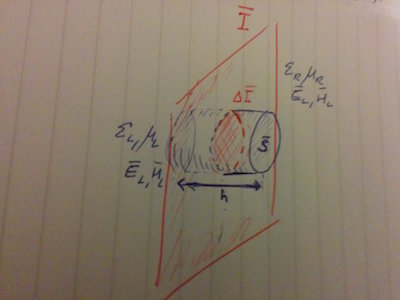
\includegraphics[height=0.3\textheight]{Figures/Chapters/PhysicalProblem/interfaceEPillBox}
  \end{center}
  \caption{Schematic showing integration surfaces used to obtain conditions for
    normal fields across an material interface.}
  \label{fig:material-interface-derivation:E-pillbox}
\end{figure}
In the limit $h \to 0$, all electric flux leaves the volume through the parallel
planes of the surface $S$, and~\eqref{eq:maxwell-gauss-integral} can be written
as
$$
\D_L \cdot \hat{\mathbf{n}} \Delta I - \mathbf{D}_R \cdot \hat{\mathbf{n}}
\Delta I = \rho_s \Delta I.
$$
The material interface condition can be written as
$$
\D_L \cdot \hat{\mathbf{n}} - \mathbf{D}_R \cdot \hat{\mathbf{n}} = \rho_s .
$$
Note that in the case where $\rho_s = 0$, meaning that there are no free
(unbound) charges, then the normal component of the electric flux density, $D$,
is continuous across the interface. By following the analogous procedure for the
magnetic field using~\eqref{eq:maxwell-gauss-magnetism-integral} a similar condition is obtained
$$
\B_L \cdot \hat{\mathbf{n}} = \B_R \cdot \hat{\mathbf{n}} .
$$
These conditions are used with Maxwell's divergence equations.
% TODO F - ruben said this isn't clear....I'm not sure I fully understand them either...
% not used in the code!?

\subsection{Tangental fields}

Consider a closed rectangular integration path, $P$, perpendicular to $I$ in the plane of $\E_L$ and $\E_R$ as shown in~\eqref{fig:material-interface-derivation:E-rectangular-loop}.
\begin{figure}[htbp!]
  \begin{center}
    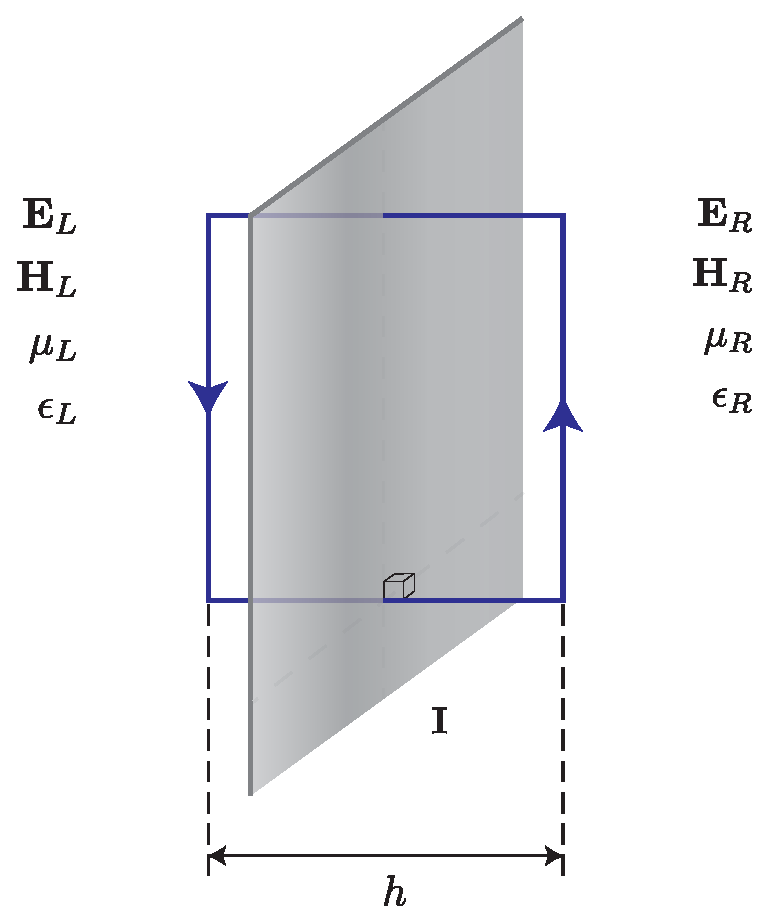
\includegraphics[height=0.3\textheight]{Figures/Chapters/PhysicalProblem/interfaceContour}
  \end{center}
  \caption{Schematic showing integration contours used to obtain conditions for
    tangental fields across an material interface.}
  \label{fig:material-interface-derivation:E-rectangular-loop}
\end{figure}
In the limit $h \to 0$ and noting that $d\maxwellSource = 0$, equation~\eqref{eq:maxwell-faraday-integral} can be written as
\begin{equation}
  \label{eq:material-interfaces-tangentalcondition-E}
  \int_{L_1}^{L_2} \E_L \cdot d\mathbf{l} - \int_{R_1}^{R_2} \E_R \cdot d \mathbf{l} = 0
\end{equation}
or
$$
\E_L \cdot d\mathbf{l} = \E_R \cdot d \mathbf{l} .
$$

The resulting interface condition is therefore that components of $\E$ tangental to the interface are continuous, or more generally
$$
\hat{\mathbf{n}} \times \E_L = \hat{\mathbf{n}} \times \E_R .
$$
Again following an analogous procedure for the magnetic field results in
$$
\hat{\mathbf{n}} \times \H_L = \hat{\mathbf{n}} \times \H_R .
$$
These conditions are used with Maxwell's curl equations.
% TODO F - again ruben said prev sentence isn't clear....I'm not sure I fully understand them either...

\subsection{Perfect electric conductors}
Metals with a large number of conduction band electrons can be described by the
perfect electric conductor (PEC) approximation. In a PEC the coulomb repulsion
between electrons causes all free charges to be distributed in an
infinitesimally thin layer on the surface of the material. The distribution of
free charges within a PEC changes instantaneously to counteract any applied
electric fields. Let us consider that the material on the right hand side of the
interface described above is a PEC. In this case, since $E_R$ is zero inside the
material, then~\eqref{eq:material-interfaces-tangentalcondition-E} simply
becomes
\begin{equation*}
\int_{L_1}^{L_2} \LMat{E} \cdot d\mathbf{l} = 0 ,
\end{equation*}
% TODO: L1 and L2 not defined
and the resulting condition is
\begin{equation}
\LMat{E} \times \hat{\mathbf{n}} = 0 .
\label{eq:material-interfaces-tangentalcondition-E-PEC}
\end{equation}
A similar procedure for the magnetic field results in
\begin{equation}
\outnormalvector \cdot \LMat{H} = \J_s ,
\label{eq:material-interfaces-tangentalcondition-H-PEC}
\end{equation}
where $\J_s$ is the surface current.

In the $TEz$ mode, only is automatically satisfied and the
boundary conditions
% TODO - what about the other two conditions i.e. divergence conditions - should
% I specify those too?
% VIVA: what does this mean? According to Ruben/Oubay paper: the tangiental
% component of the electric field vanishes at the surface of the PEC

\subsection{Radiation condition}
Solution of many problems of interest require computation of phenomena occuring
in a physical domain of infinite extent. In such an infinite domain, electromagnetic
sources are all considered to be at the origin, and to scatter energy to infinity.
A condition is required to prevent the non-physical inverse process, where energy
is transferred by radiation from infinity to the origin, and ensure uniqueness of
the solution in an infinite domain. The following condition,
known as the \SilverMuller radiation condition, must be satisfied
% TODO F - reference for Silver-Muller radiation
\begin{align}
  \lim_{ r \to \infty } \left( \xbf \times \left( \nabla \times \E \right) + \left| \xbf \right| \dpartt{\E} \right) = \mathbf{0}, \\
  \lim_{ r \to \infty } \left( \xbf \times \left( \nabla \times \H \right) + \left| \xbf \right| \dpartt{\H} \right) = \mathbf{0}.
\end{align}
% VAIVA - do I understand this?
% TODO F - Lots of things circled here...check them all...!

\section{Relation to wave equation and Helmholtz equation}
\subsection{Wave equation}

Within a homogenous medium, where material parameters are constant and no free currents or charges are present, Maxwell's equations can be written in wave equation form, for which plane wave analytical solutions can be obtained~\cite{Jackson:490457}. Substitution of the constitutive relations for linear media,~\eqref{eq:constitutive-linear}, into Faraday's law,~\eqref{eq:maxwell-ampere}, without no free charges ($\rho = 0$), results in the expression
\begin{equation}
  \label{eq:wave-equation-derivation-1}
  \nabla \times ( \nabla \times \H ) + \eps_0 \eps_r \dpartt{ \left( \nabla \times \E  \right) } = 0 .
\end{equation}
Substitution of the vector identity, $ \nabla \times ( \nabla \times \H ) = \nabla \cdot ( \nabla \cdot \H ) - \Delta \H $, into~\eqref{eq:wave-equation-derivation-1}, and noting from~\eqref{eq:maxwell-gauss-2} that $\nabla \cdot \H = 0$, when $\rho = 0$, results in
\begin{equation}
 \Delta \H = \eps_0 \eps_r \dpartt{ \left( \nabla \times \E  \right) } = 0 . \label{eq:wave-equation-derivation-2}
\end{equation}
Substitution of Ampere's law,~\eqref{eq:maxwell-ampere}, into~\eqref{eq:wave-equation-derivation-2}, results in
\begin{equation}
  \label{eq:maxwell-wave-eqtn-H}
  \Delta \H = \frac{1}{c^2} \ddpartt{ \H },
\end{equation}
which is a wave equation in the unknown $\H$, with the speed of the wave given by $\speedoflight = 1/\sqrt{\eps_0 \eps_r \mu_0 \mu_r }$. Note that the quantities $\eps_0$ and $\mu_0$ are related to the speed of light in vacuum $c_0 = 1/\sqrt{\eps_0 \mu_0 }$. Starting from Ampere's law, and following a similar procedure with no free currents ($ \J = 0 $), results in
\begin{equation}
  \label{eq:maxwell-wave-eqtn-E}
  \Delta \E = \frac{1}{c^2} \ddpartt{ \E } .
\end{equation}
% TODO - Ruben : comments are missing - what are the advantages/limitations of
% this formulation!! Look at LeVeque - why do use conservation laws in this
% way?

\subsection{Helmholtz equation}
The Helmholtz or reduced wave equation form of~\eqref{eq:maxwell-wave-eqtn-E} is obtained by assuming the fields $\E$ and $\H$ are time-harmonic, expressed as
\begin{align}
  \label{eq:maxwell-helmholtz-time-harmonic-soltn}
  \E(\xbf,t) = \Re \left( \EHelm(\xbf) e^{i \omega t} \right), \\
  \H(\xbf,t) = \Re \left( \HHelm(\xbf) e^{i \omega t} \right),
\end{align}

Substitution of~\eqref{eq:maxwell-helmholtz-time-harmonic-soltn} into the wave equations, ~\eqref{eq:maxwell-wave-eqtn-E} and~\eqref{eq:maxwell-wave-eqtn-H}, results in the Helmholtz equations for electric and magnetic fields,
\begin{align}
  \label{eq:helmholtz}
  \Delta \E(\xbf) + k^2 \E(\xbf) = 0, \\
  \Delta \H(\xbf) + k^2 \H(\xbf) = 0,
\end{align}
where $k^2 =\omega^2/c^2$, is the propagation constant and the speed of the electromagnetic radiation is given by $c$. In this form the equations for $\E$ and $\H$ can be solved independently for each angular frequency, $\omega$. This approached is best suited to problems with a small, known number of frequencies of interest, for example a system which is being driven at a known frequency. By contrast the time domain approach allow solution for a broad band of frequencies at once.


% TODO Balanis citation is incomplete P Drude - needs to be removed - maybe the
% solid state one (Optical properties of solids) instead Maybe swap some of the
% references for others (e.g. Fox) Ruben made LOADS of comments on citations Use
% some citations from Rubens paper also


%%% Local Variables:
%%% mode: latex
%%% TeX-master: "../Thesis"
%%% End:
